\documentclass[10pt, twocolumn]{article}
%nobalancelastpage

\usepackage{labreportstyle}
\usepackage{listings}
\graphicspath{{../images/}}

\lhead{M. Rossetter}
\rhead{Interquark Potential Modelling of Charmonium}
\title{Interquark Potential Modelling of Charmonium}
\author{M. Rossetter \\ Physics Problem Solving Computing Project}
\date{\vspace{-0.30cm} \today}

\begin{document}
\twocolumn[
\maketitle
\begin{onecolabstract}
    \vspace{-20pt}
    A study using interquark potential models to replicate the bound masses of charmonium and gain insight into the strong force interaction. 
    Two potentials, the Cornell potential and a quasilogarithmic form, were considered, both yielding successes and failures over different distances, communicating an understanding of the strong interaction in these regions. 
    Hyperfine splitting of S states is also considered, and it is concluded that without relativistic effects, these states cannot be accurately replicated.
\end{onecolabstract}]
\thispagestyle{plain}

\section{Introduction}
This study will use the quarkonium system of the charm quark, known as charmonium, as a means of studying how to model the interquark potential generated by the strong force.
Due to the complex nature of the strong force, it is difficult to study strong force processes using standard methods in many cases. 
The interactions of the strong force at very small distances ($<0.5\,fm$) and large distances ($\sim2\,fm$) are well characterised, but a single description over all distances, and the intermediary distances, has not yet been devised. \\
The strong force generates bound systems of three quarks (baryons) or one quark and an anti-quark (mesons). 
Studying mesons is an integral part of learning about the strong force as it provides a much simpler case than the three-body systems of baryons, and can be used to build up knowledge of the strong force before applying it to more complicated systems. 
Quarkonia, the mesons formed of a quark and its own flavour anti-quark, provide the simplest mesons to study in the case of the heavier quarks, where asymptotic freedom comes into play and the strong coupling constant, $\alpha_s$, is small enough that perturbation theory can be used to study these systems \cite{3}.
From these requirements, the quarkonia most suited to study are charmonium and bottomonium, as their masses lie within the asymptotic freedom regime and unlike toponium, their lifetimes are long enough that they can feasibly be studied.
For this study, the approximation that relativistic effects are negligible for charmonium is used, which can be confirmed by estimates of quark velocities. \\
The best way to study charmonium for insights into the strong force is through spectroscopy of its energy levels, or bound mass levels, as these are often easier to compare to experiment. 
The bound masses of charmonium have been measured often in experiment and mostly have well-known values. 
From a theoretical approach, the wavefunction for different charmonium states can be found and the mass of the system calculated from this. 
This approach will require using an interquark potential, which must be modelled using known expectations of the behaviour of the strong force in this interaction. 
The choice of interquark potential is an important one for finding the bound masses of charmonium, and the accuracy of these masses to measurement indicates the validity of the potential, which in turn reinforces the phenomenological interpretations of the strong force interaction that give rise to the potential.

\section{Non-Relativisic Potential Modelling}
An issue with modelling charmonium is that there is no potential that can be simply derived like in electromagnetism, as there is no uniform theory for the interaction across the range of radii considered.
Theoretical descriptions of quark interactions confine certain aspects of potential models, expecting certain behaviours as $r$ tends either to $0$ or $\infty$.
Any potential models considered are then phenomenological, and will differ in how their creators choose to interpret experiment and describe the potential uniformly based on the behvaiour at small and large distances.
These phenomenological models will never be wholly accurate to the real potential that is at work, but some may describe quarkonia systems to a practical accuracy for some states.\\
An interquark potential is expected to have a Coulomb-like part to prevent the quarks from getting too close to each other and annihilating, as well as a linear growth part which confines the quarks to the system and prevents them from becoming free particles.
These two parts are brought together in the first model which will be used in this study - the Cornell potential \cite{3},
\begin{equation}
    V_1(r) = -\frac43\frac{\alpha_s}{r} + \beta r,
\end{equation}
where $\frac43$ is derived from colour charge, $\alpha_s$ is the strong coupling constant whose value is dependent on the mass of the quarks being considered, and $\beta$ is a constant to be determined. \\
The Cornell potential balances the short-range and long-range interactions in two different terms, although many other potentials try to combine both these interactions into one term through analysis of experimental data. 
A quasilogarithmic potential,
\begin{align}
    V_2(r) &= cr^d + b,
\end{align}
is one such potential that is derived from the interpretation of colour confinement in quarks and approximate constant that is the splitting of the $2^3S_1$ and $1^3S_1$ states in charmonium and bottomonium \cite{2}. 
$c,d,$ and $b$ are arbitrary constants of the model. \\
Equations (1) and (2) are the potentials used in this study, although there are many other models known for their success, some of which will be discussed in Section \RN{8}.

\section{Finding the Charmonium Wavefunction}
The spin-averaged wavefunction for charmonium will satisfy the 3D Schrodinger equation,
\begin{equation}
    -\frac{\hbar^2}{2\mu}\nabla^2\psi + \left[V(r) - E_{nl}\right]\psi = 0,
\end{equation}
where $\mu = \frac{m_c}{2}$, and $m_c$ is the mass of a charm quark.
Through separation of variables, $\psi = R_{nl}Y^m_l$, the radial wavefunction, $u_{nl} = rR_{nl}$, can be simplified into a set of first order ODEs, 
\begin{align}
    \frac{du_{nl}}{dr} &= v_{nl}, \\
    \frac{dv_{nl}}{dr} &= \frac{l(l+1)}{r^2}u_{nl} - 2\mu\left[E_{nl} - V(r)\right]u_{nl},
\end{align}
These can then be solved for $u_{nl}$ for each energy eigenstate.
Boundary conditions must be set in the limit as r tends to 0.
Ignoring normalisation for now, we require that
\begin{align}
    u_{nl}(0) &= 0, \\
    \frac{du_{nl}(0)}{dr} &= 1.
\end{align}
Once $u_{nl}$ has been solved, it is normalised such that
\begin{equation}
    \int_0^\infty r^2|R_{nl}|^2dr = \int_0^\infty |u_{nl}|^2dr = 1.
\end{equation}
Experiment measures the mass of charmonium states rather than their energies, so it is easier to use the masses for comparison.
For a spin-averaged quarkonia energy $E_{nl}$ and a quark mass $m_q$, the spin-averaged bound mass \cite{1},
\begin{equation}
    M_{nl} = E_{nl} + 2m_q.
\end{equation}

\section{Methodology}
A program was written using Python to solve the Schrodinger equation as discussed in Section \RN{3}, using initial estimates for $E_{nl}$, and normalised using Simpson's method.
Equations (4) and (5) were put into scipy.integrate's odeint function to solve for $u_{nl}$. 
The array of values for the radius must start slightly away from 0 due to numerical inaccuracies in the solver.
In reality, the wavefunction should be able to decay to zero as $r\to\infty$, but for numerical solutions, a limit to $r$ must be set. 
For most charmonium states, it is recommended that $r \leq 15\,\text{GeV}^{-1}$.
Due to the nature of the solution, most energies will diverge to $\pm\infty$, and only the correct energy for the particular $(n,l)$ state will yield a solution that abides by the requirements of normalisation.
To find the correct energy, the bisection method was used.
The program was first tested on the simpler case of the Hydrogen atom, before being applied to charmonium.

\subsection{Bisection Method}
The bisection method finds the wavefunction for initial guesses of energies and iterates over the range of these to find the correct value for the energy of the particular spin-averaged eigenstate, $E_{nl}$.
Two initial energies are guessed, defining a range between them where the correct energy is believed to lie.
A third energy is then calculated as $E_2 = \frac12 (E_1+E_3)$.
For each of these energies, the wavefunction's nodes and turning points are counted - for a quarkonium wavefunction $u_{nl}$, there will be $(n-1)$ nodes and $n$ turning points.
If this is not the case for any of the particular energies used, then new energies must be tried. 
If the number of nodes and turning points differs between two of the three energies, then the correct energy will be somewhere between these two. 
These two energies are set as the new $E_1$ and $E_3$, and the process is performed again.
This method is repeated until the energies converge on an energy with the correct nodes and turning points, which will be $E_{nl}$.

\subsection{Hydrogen Wavefunction}
To test the functionality of the program, it was first applied to the case of the Hydrogen wavefunction. 
Using $V_1$, this can be found precisely with a working version of this program, using the following changes from the problem for charmonium:
\begin{equation}
    \frac43 \alpha_s \to \alpha=\frac{1}{137},\; \beta \to 0,\; \mu \to m_e.
\end{equation}
Further to this, the radial distances considered here limit the maximum values used to $5200 \leq r_{max} \leq 9500\,\text{MeV}^{-1}$ for increasing energy levels.
Unlike charmonium, the energy levels of Hydrogen are not dependent on the azimuthal quantum number, $l$, so for its wavefunction $u_{nl}$, it will have $(n-l-1)$ nodes and $(n-l)$ turning points.
The precise solutions for the energy levels of Hydrogen should follow, confirming the program to be ready for charmonium.

The bisection method was then applied to the charmonium wavefunction for both $V_1$ and $V_2$, and the spectra of the bound states was developed for both potentials. 
The found energies were converted using Equation (9) into spin-averaged masses for the 1S, 1P, 2S, 2P, and 3S states of charmonium. 
For these calculations, the values of the constants in both potentials must first be found, which is discussed in Section \RN{5}.

\subsection{Hyperfine splitting of S states}
For many lower energy states, the accuracy of most potential models for spin-averaged $(n,l)$ states will be relatively high. 
A further comparison into their suitability can be found through considering the hyperfine splittings between the spin states of each $(n,l)$ system. 
Hyperfine splitting of states where $l\neq0$ becomes quite complicated, so only the $l=0$, or S, states were considered for hyperfine splitting in this study. 
For an S state wavefunction, the difference in energy/mass between the two split states is
\begin{equation}
    \Delta(n^3S_1 - n^1S_0) = \frac{8\pi\alpha_s}{9m_q^2}|R_{nl}(0)|^2.    
\end{equation}
\cite{1} The program being used here used $u_{nl}$, not $R_{nl}$, so an approximation must be made in the limit of $r\to0$:
\begin{equation}
    \lim_{r\to0} R_{nl}(r) = \lim_{r\to0} \frac{u_{nl}(r)}{r} = \frac{du_{nl}(0)}{dr}.
\end{equation}
Knowing the value of this splitting then, the $n^3S_1$ and $n^1S_0$ masses can be found from the spin-averaged mass, $M_{nl}$, using the following \cite{1}:
\begin{align}
    M_{nl}(n^3S_1) &= M_{nl} + \frac14\Delta(n^3S_1 - n^1S_0) \\
    M_{nl}(n^1S_0) &= M_{nl} - \frac34\Delta(n^3S_1 - n^1S_0)
\end{align}
The masses of $n^3S_1$ and $n^1S_0$ states are well documented, so calculating these provides further means of checking the accuracy of potential models to experiment. 
As the splitting depends on $\frac{du_{nl}}{dr}$ at 0, the accuracy of these splittings may not be connected to the accuracy of the spin-averaged masses; even if the radial wavefunction appears to be solved correctly and yields a good value of spin-averaged mass, values of the wavefunction at certain points (i.e. at 0) may be different from reality, meaning that the hyperfine splitting values could still be broadly inaccurate.
$\frac{du_{nl}(0)}{dr}$ is important in the analysis of wavefunctions, yielding hyperfine splittings as well as the lifetime or "width" of the system \cite{1}. 
Using calculations involving this can provide further insight into validity of solutions; the further the hyperfine splitting deviates from theory, the less viable the solutions must be, even if their spin-averaged masses are accurate.

\section{Calculating Parameters}
The parameters of the two potentials have many values documented in literature that could be used, but these will vary depending on the value of the charm quark mass used; here $m_c = 1.34\,\text{GeV}/c^2$\cite{11}. 
Values from literature could be used, but the accuracy of the calculation of the masses would suffer, if converging solutions could be found at all.\\
The initial method considered was using the bisection method, using the known value of the spin-averaged charmonium ground state, $M_{10} = 3.068\,\text{GeV}/c^2$ \cite{10}, and varying over the unknown constant instead of energy.
This method can work well for $V_1$ as $\alpha_s$ can easily be fixed from literature for whichever value is chosen for the charm mass. 
Once $\beta$ is found from the bisection method, the potential is fully known and can be used in the bisection method to find energies. \\
However, when considering $V_2$, it is clear that this method will likely be less accurate.
Unlike $V_1$, where $\alpha_s$ is derived from something more than just the model, all three parameters of $V_2$ are arbitrary and will always be specific to each paper recording their values, so setting two of these values as constants from literature could never be seen as a true calculation of this potential for the mass of charm quark being studied.\\
From considering the limitations with $V_2$, another method for finding the parameters was considered. 
Using initial guesses of parameters in the range of literature values, the function applying the bisection method over energy was put into scipy.optimise's minimise package, requiring it to find the optimum potential parameters to minimise the difference between the known ground state energy and the found ground state energy. \\
This method will hold no bias for one potential over another, and should optimise all parameters equally, such that the parameters will be balanced when solving the ground state energy rather than giving more significance to either the small or large distance limit, as could happen with the first method, leading to particular cases of higher or lower accuracies in different distance regimes.
The accuracies of the masses should instead be reflected over the whole potential, with a natural drop off due to additional phenomena not considered in this study, such as increasing relativistic effects for higher states which will be discussed in Section \RN{7}.
Optimising in this way, the parameters follow as:
\begin{align}
    V_1 &:\; \alpha_s = 0.401,\, \beta = 0.195 \\
    V_2 &:\; c = 7.641,\, d = 0.102,\, b = 8.061.
\end{align}
For $\beta,d,$ and $b$, these values are close to what would be expected from literature, with slight deviations that were expected and anticipated due to the different specifics of this study from any other. 
It was expected that $\alpha_s = 0.4$, which is extremely close to what is derived, with the optimiser agreeing that the theoretical value is what the coupling constant should be for the charm mass used.\\
There is a more significant deviation from literature for $c$, deviating by $\sim 16\%$.
Although this is relatively large, it is not significant enough to warrant questioning the method; for $V_2$, $d$ and $b$ are less likely to change much depending on mass, as $d$ gives the potential its shape which should remain the same for all masses, and $b$ is a threshold for the potential at $r=0$ which again will be less dependent on charm mass. 
However, $c$ will dictate the magnitude of the curve as it continues away from 0 - this value will be expected to change more with the charm mass. 

\section{Results}
Following the method discussed above, the program was tested by solving the Hydrogen wavefunction. 
Solutions were sought for 1S, 2S, 2P, and 3S states; these are shown in Figure 1, and as can be seen, the program was successful in this test, replicating the energy levels of Hydrogen comfortably. 
\begin{figure}[H]
    \centering
    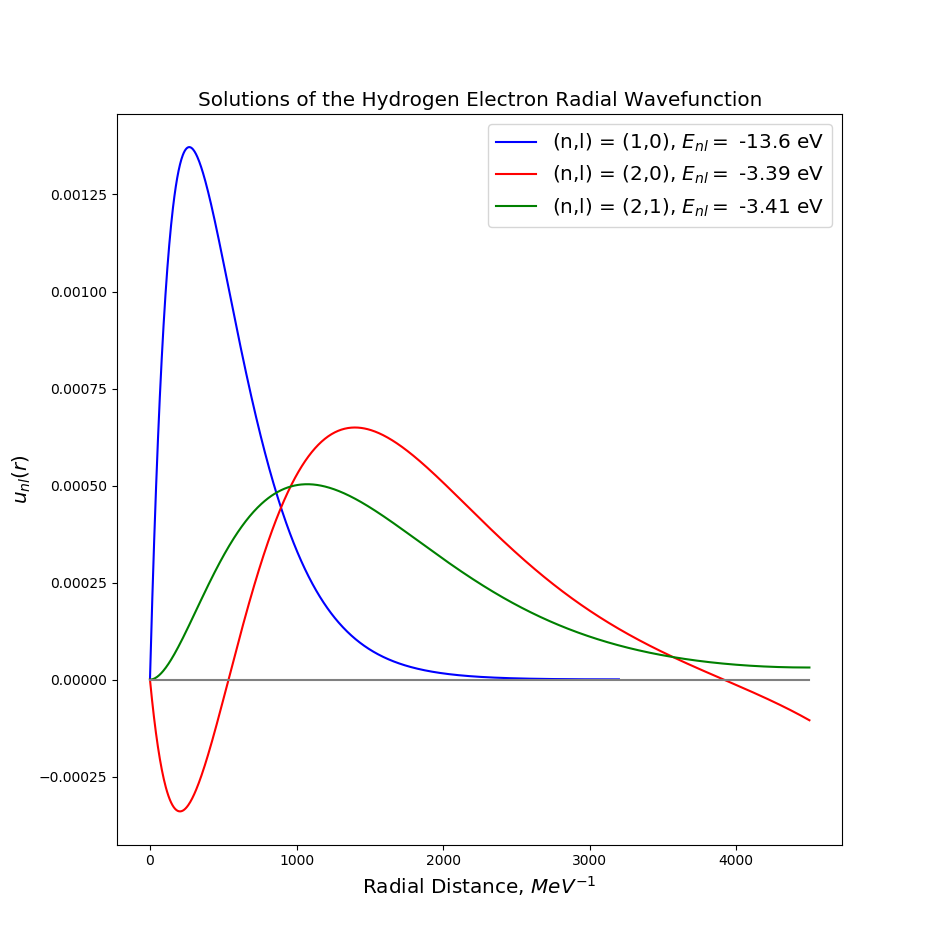
\includegraphics[width=0.45\textwidth]{Hydro}
    \caption{A plot of solutions for radial wavefunction for Hydrogen for the 1S, 2S, 2P and 3S states, using the bisection method to find the energies.}
\end{figure}
The energy levels found are presented in the figure to 3 significant figures, as this was the accuracy to which input values were quoted. \\
As discussed in Section \RN{5}, once the program was confirmed for Hydrogen, the first thing towards solving for charmonium is to find the values for the parameters of the two potentials. 
The values of these parameters are found in Equations (15) and (16).
\begin{table}[H]
    \vspace{7pt}
    \centering
    \begin{tabular}{|c|c|c|c|}
        \hline 
        \rowcolor{lightgray} State & $V_1$ & $V_2$ & Experiment \\
        \hline
        1S & $3.068$ & $3.068$ & $3.068$ \\
        \hline
        1P & $3.522$ & $3.557$ & $3.525$ \\
        \hline
        2S & $3.717$ & $3.745$ & $3.649$ \\
        \hline
        2P & $4.025$ & $4.008$ & $3.993$ \\
        \hline
        3S & $4.197$ & $4.139$ & $4.028$ \\
        \hline
    \end{tabular}
    \caption{The calculated masses of the spin-averaged bound states of charmonium for both potentials used in comparison to experiment\cite{6,7,10}. All masses are standard units of GeV$/c^2$.}
\end{table}
With parameters defined, the program solved for the 1S, 1P, 2S, 2P, and 3S energy levels of charmonium for $V_1$ and $V_2$.
The radial wavefunctions found are shown in Figures 2 and 3 for potentials $V_1$ and $V_2$ respectively. 
Both potentials are shown to be able to replicate wavefunctions comfortably for all states chosen, confirming that the potentials do have some physical meaning, although their precise accuracy must be determined.
The bound masses found and their experimental value are shown in Table 1 so that trends in their accuracy can be analysed. 
These are quoted to 4 significant figures as it was decided that more precision was required in the hope that the calculated states could come near to the measured results.
It was expected that the agreement with experiment would drop off as masses increased due to rising relativistic effects, which can be seen in the table. 
\begin{figure}[H]
    \centering
    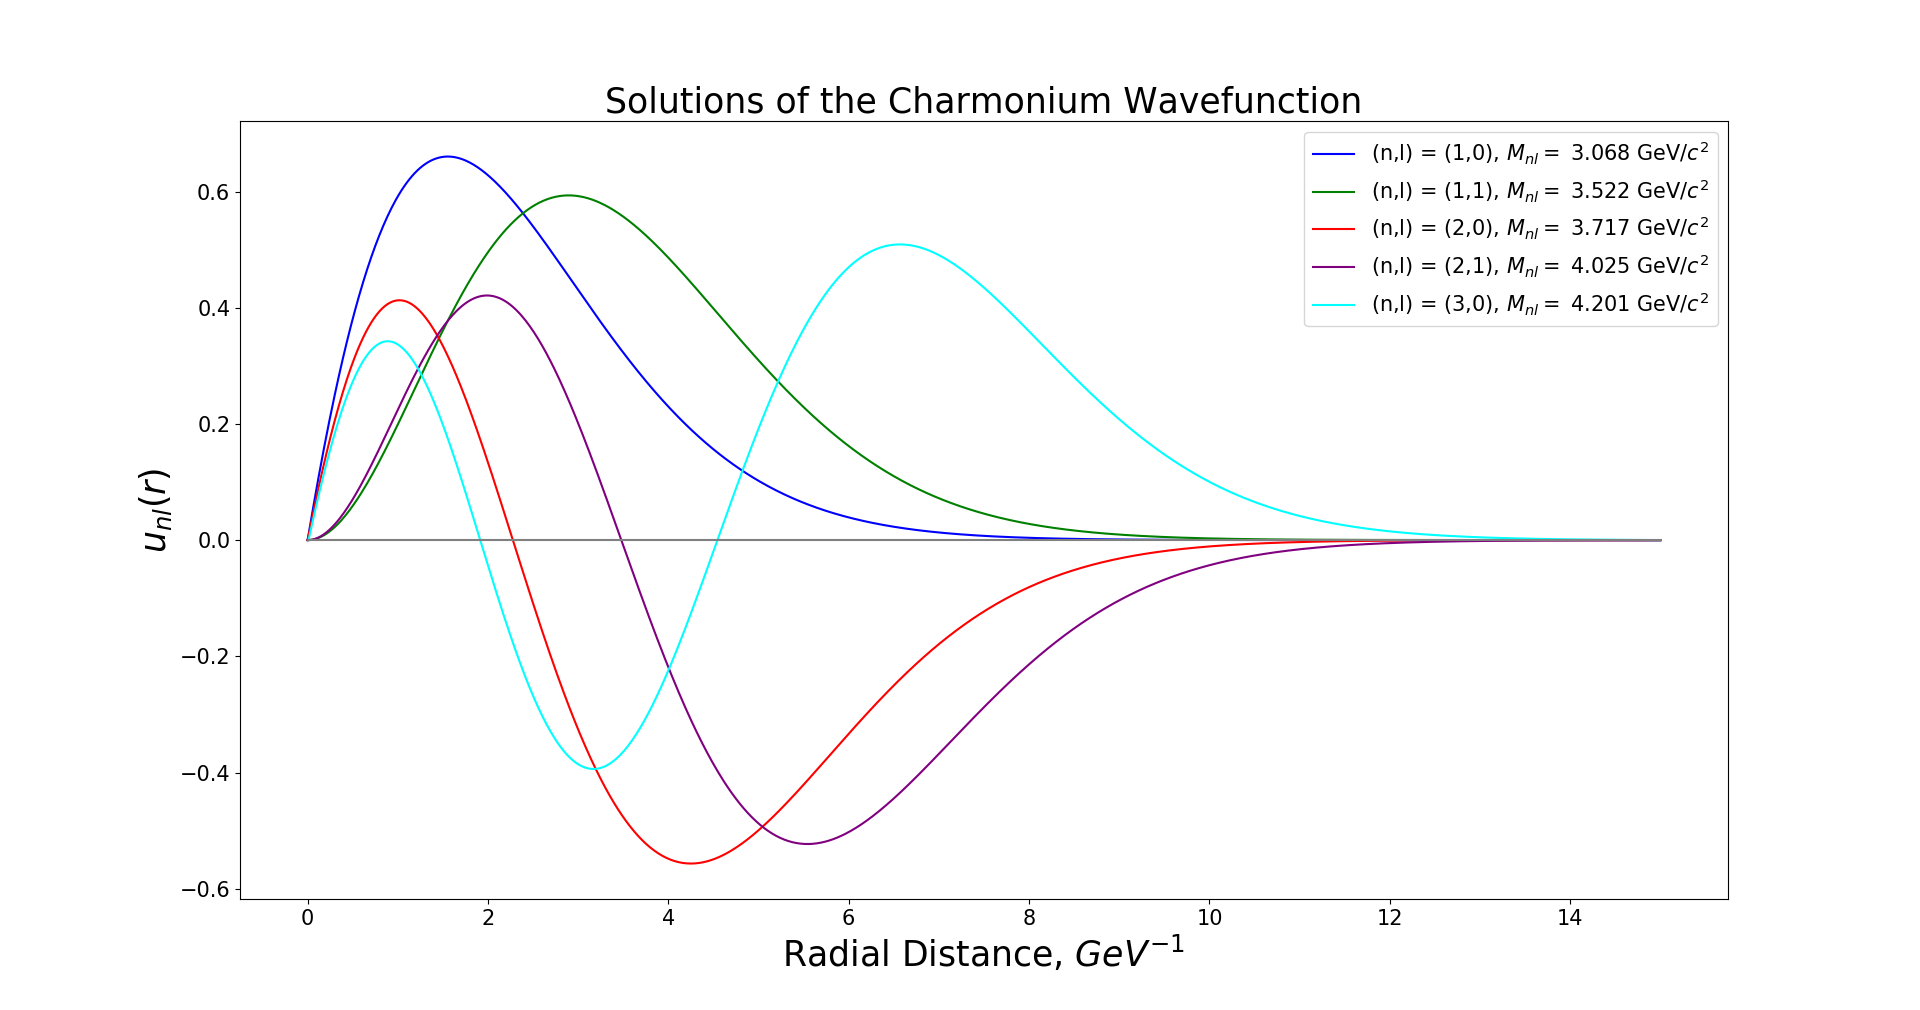
\includegraphics[width=0.45\textwidth]{fullspec}
    \caption{Spin-averaged radial wavefunctions for 1S, 1P, 2S, 2P, and 3S states using $V_1$. The masses of these states were calculated using Equation (9) from the energies found from the bisection method.}
\end{figure}
\begin{figure}[H]
    \centering
    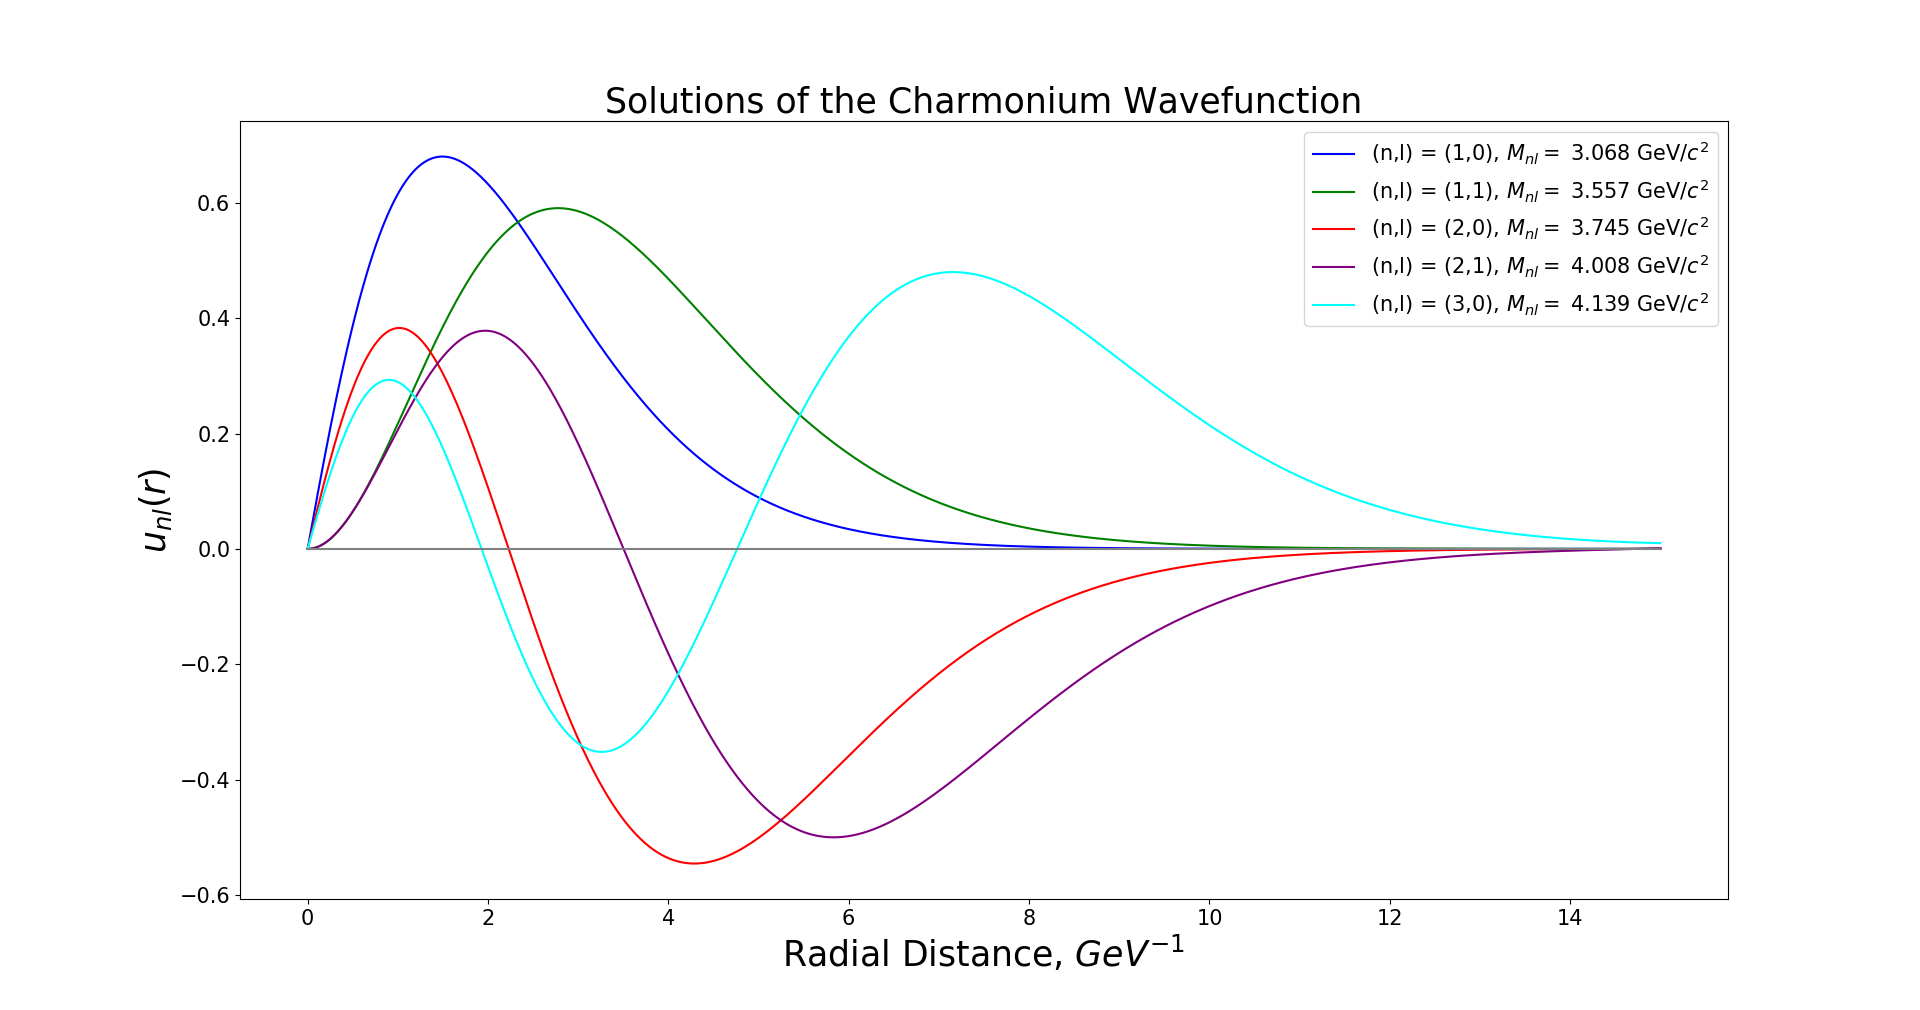
\includegraphics[width=0.45\textwidth]{fullspec2}
    \caption{Spin-averaged radial wavefunctions for 1S, 1P, 2S, 2P, and 3S states using $V_2$. The masses of these states were calculated using Equation (9) from the energies found from the bisection method.}
\end{figure}
Due to the potential parameters being optimised for the ground state energy, the values found for these are naturally accurate to the value of experiment, at least to the precision of the project.
The other states, as expected for both potentials, diverge from the experimental values as they go up in energy. 
Initially, $V_1$ is more accurate to experiment over 1P and 2S, but is less accurate than $V_2$ for 2P and 3S. 
This can be interpreted from the functionality of the two potentials: $V_1$ must be a more accurate potential in the smaller distance limit, whereas $V_2$ must be more accurate in the larger distance limit. 
This interpretation will be expanded in Section \RN{7}.\\
After finding the spin-averaged masses, the hyperfine splitting of S states was calculated and the different split S states were found; these are tabulated in Table 2 with the experimental values for comparison.
\begin{table}[H]
    \vspace{10pt}
    \centering
    \begin{tabular}{|c|c|c|c|}
        \hline
        \rowcolor{lightgray} State & $V_1$ & $V_2$ & Experiment \\
        \hline
        $1^1S_0$ & $2.576$ & $2.630$ & $2.980$ \\
        \hline
        $1^3S_1$ & $3.232$ & $3.214$ & $3.096$ \\
        \hline
        $2^1S_0$ & $3.375$ & $3.502$ & $3.638$ \\
        \hline
        $2^3S_1$ & $3.831$ & $3.826$ & $3.686$ \\
        \hline
        $3^1S_0$ & $3.898$ & $3.965$ & $4.020$ \\
        \hline
        $3^3S_1$ & $4.297$ & $4.197$ & $4.040$ \\
        \hline
    \end{tabular}
    \caption{Masses of $n^3S_1$ and $n^1S_0$ states for $n = 1,2,3$ from hyperfine splitting. The masses calculated from both potentials are compared to the ones found in experiment \cite{4}.}
\end{table}
For all hyperfine states, $V_2$ is seen to be the more accurate of the two potentials, although both potentials suffer from having much larger separations from the spin-averaged mass. 
This is indicative that although the potentials used can come close to finding the spin-averaged masses, when taking into consideration things such as the hyperfine interaction, the potentials fall away from reality. 
The defining factor for the hyperfine splitting is the value of the wavefunction at 0. 
Although the wavefunctions and spin-averaged masses found in this study are broadly successful, the specific value of the wavefunction at 0 is not accurate to reality, else the hyperfine states would be more accurate. 
This could be due to a number of factors, but is most likely due to normalisation issues - either that the magnitude of the function was different from what it should be due to the variation in state energy, or that the method of normalisation itself is flawed to some degree.

\section{Discussion}
\subsection{Success and Failure of Potentials}
For spin-averaged masses, both potentials came close to the measured values from experiment, although with some deviation, as shown in Tables 1 and 2.
The parameters were defined using the ground state mass, so both potentials can perfectly replicate the wavefunction and the mass for the ground state, but for other states, the models deviate from experiment by different amounts. \\
$V_1$ is found to be more accurate for the lower energy states, 1P and 2S. 
This is likely due to difference between the Coulomb-like and linear parts of the potential. 
The Coulomb-like part describes the short range interaction of the strong force by direct analogy to the electromagnetic potential, using constants with known physical meaning, such that for short ranges, this part of the potential is likely to be extremely accurate and deviations from this are due to the extra factor of the linear term. 
As the radial distance increases, the linear term becomes more dominant, and the calculated bound mass becomes larger than experimental values. 
The simplest interpretation that immediately reveals itself is that the linear term increases more rapidly than it realistically should. 
Perhaps changing this term to $\beta r^\gamma$, where $0 < \gamma < 1$ would still provide the increasing part categorised in the linear term, but would increase at a slower rate.
Even for the lower energy states, having a smaller linear term could decrease the found energies and yield greater accuracy. \\
For $V_2$, the opposite problem presents itself. 
It becomes more accurate for the higher states, 2P and 3S, and is less so for lower energy states. 
It is more difficult to break down this potential as it is all confined into a single term.
However, by analogy to the break down of $V_1$, it can be seen that this potential works better in the longer (or at least intermediary) distances, characterising the linear-like expectancy for colour confinement more than the Coulomb-like part for closer distances. \\
Even for the more accurate higher masses, the solved masses are all greater than the experimental values. 
This suggests the potential is generally set higher than it should be in reality. 
It is likely that this is due to either both or one of the values of $b$ and $c$ are higher than they should be to properly model. 
If it is the case that this potential is stronger for modelling higher states, then perhaps optimising the parameters for the ground state energy was in contradiction to the nature of the potential.  Optimising using another energy level, such as 3S for example, might prove a more accurate potential.

\subsection{Interpretation from Hyperfine Splitting}
As discussed above, the potentials both warranted some accuracy for different energy regions for spin-averaged states. 
However, when considering the results of the hyperfine splitting, it is clear that $V_2$ recreates the conditions for this splitting more accurately, although both potentials have far larger splittings than expected.
The value of $\frac{du_{nl}(0)}{dr}$ is the key factor in determining this splitting. 
For the $n^1S_0$ and $n^3S_1$ states to be smaller and larger respectively than experiment, $\frac{du_{nl}(0)}{dr}$ must be larger than it should be. 
The simplest explanation of this would be either an error in the method of normalisation or that the wavefunction was of a slightly higher magnitude overall than expected.
The latter of these is more likely to have a significant effect as the error in Simpson's method for integration is negligible for the level of accuracy considered here. 
By analysis of Figures 2 and 3, or specific analysis of $\frac{du_{nl}}{dr}$ for the spectra of both potentials in Figure 4, it is seen that the wavefunctions are initially much steeper for $V_1$ than $V_2$, so for $V_2$, $\frac{du_{nl}(0)}{dr}$ is smaller for all states.
\begin{figure}[H]
    \centering
    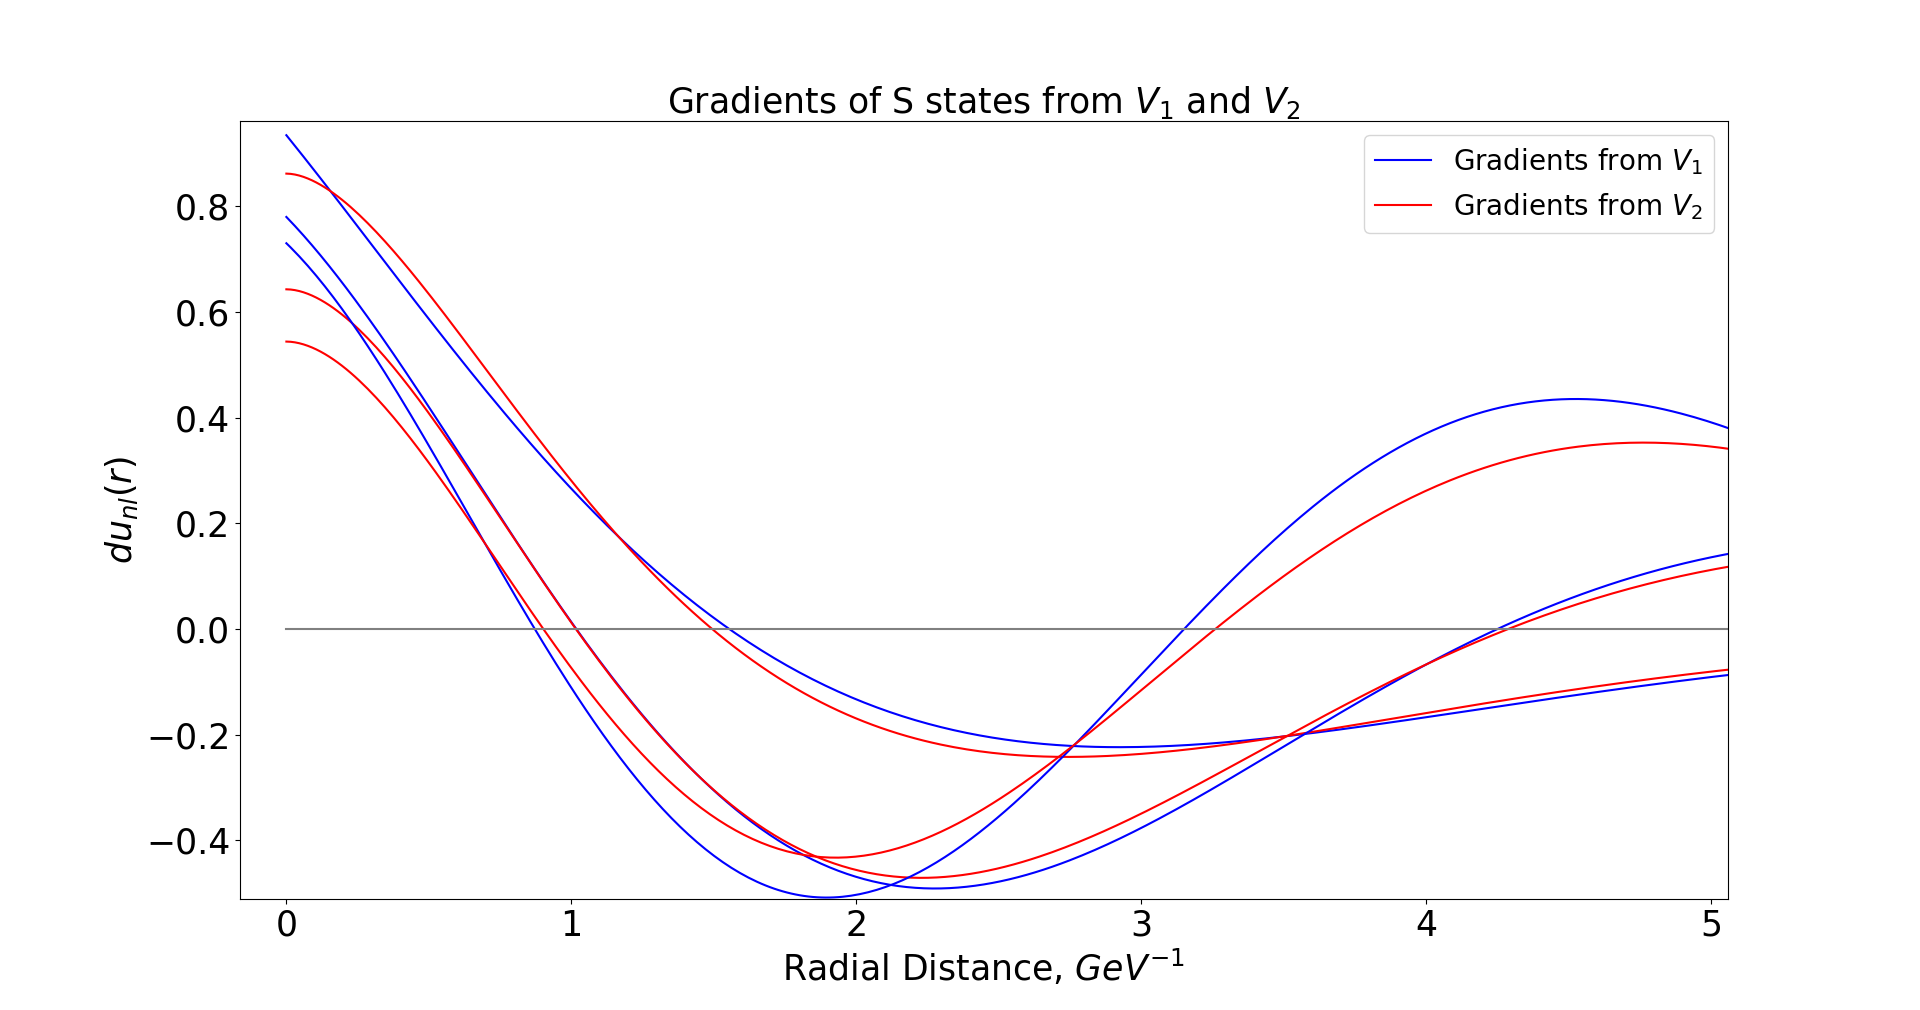
\includegraphics[width=0.45\textwidth]{grads}
    \caption{A plot of the S state gradients near the origin, showing that for all states, $V_2$ gives a lower value of the gradient at 0.}
\end{figure}
The gradient at 0 is as important for the real system as the bound mass is, yielding the hyperfine splitting energy separation and the lifetime of the state. 
From this, $V_2$ seems to be a more functional model, yielding more realistic hyperfine splittings, independent of the accuracy of the calculated bound mass. 
However, $V_2$ still produces significantly larger splittings than there should be. 
It is difficult to see exactly where this comes from, although it is likely that this is down the potential model again. 
Other potentials could be chosen specifically to minimise the deviation in the hyperfine splitting, but disregarding a change of potential for now, the issue presented within $V_2$ is the values of the parameters. 
Like discussed above, perhaps different optimisation methods could be used to improve the specifics of the potential model such that $\frac{du_{nl}(0)}{dr}$ would be improved and the hyperfine splitting would be closer to experiment.\\
In addition, spin interactions such as that of the hyperfine splitting are more relativistic in nature, so without including relativistic corrections to the potential, these may not be able to be replicated.

\subsection{Relativistic effects}
An important assumption made throughout this study has been that the quarks in charmonium states considered here do not move fast enough that relativistic effects need be considered such that non-relativistic quantum mechanics can be used to solve for the wavefunctions.
The validity of this assumption should be considered in order to determine the validity of the non-relativistic potentials used here.\\
An initial check for relativistic effects is velocities of the quarks found through estimations by virial theorem. 
These velocities are generally considered as being low enough that relativity need not be considered, which is one of the reasons charmonium and bottomonium are considered in the appropriate regime for these studies.\\
However, another way of looking for relativistic effects is by finding the value of the expectation value $\langle v^2/c^2\rangle$ for each state. 
The relevant values are shown in Table 3.
\begin{table}[H]
    \vspace{7pt}
    \centering
    \begin{tabular}{|c|c|c|}
        \hline
        \rowcolor{lightgray} State & J$/\Psi$ & $\Upsilon$ \\
        \hline
        1S & 0.23 & 0.077 \\
        \hline
        1P & 0.25 & 0.069 \\
        \hline
        2S & 0.29 & 0.075 \\
        \hline
        2P & 0.32 & 0.078 \\
        \hline
        3S & 0.36 & 0.085 \\
        \hline
    \end{tabular}
    \caption{The characteristic expectation value for relativistic effects, $\langle v^2/c^2\rangle$, for each of the spin-averaged states of charmonium (J$/\Psi$)  used in this study and the equivalent bottomonium ($\Upsilon$) states, as found in \cite{8}.}
\end{table}
For bottomonium, $\langle v^2/c^2\rangle$ is negligible and a non-relativistic potential is a much better approximation.
Although not extremely high, the expectation values for charmonium states are high enough such that there will be some relativistic effects. 
These effects will not be significant enough at the relatively low energy levels considered here to massively impact the spin-averaged model, but will have a slight effect for all levels, and will be partly to blame for the general decrease in accuracy to experiment as the masses increase as relativistic effects become stronger.\\
The spin interactions that cause the hyperfine splitting are more relativistic in nature as well, so with the above expectation values, there will be a large dependency of these values on relativistic effects.
Therefore, a significant portion of the inaccuracy in hyperfine model will be due to relativity not being considered in the calculation of the splitting or even the potential. \\
In summary, non-relativistic potentials are definitely a good enough approximation to get close to the experimental values, moreso for bottomonium than charmonium, but to get more accurate results, relativistic effects must be taken into account, particularly for hyperfine splitting. 

\subsection{Charm quark mass}
The charm quark mass is the only value input to the program that was not calculated or selected in some way through methods discussed above. 
There is difficulty in determining the exact free mass of a quark as it will never exist as a free particle. 
Current measurements have the best value of the charm mass as $m_c = 1.275\,$GeV$/c^2$ \cite{10}.
However, this value can vary - in different situations, there will be a different number of virtual gluons and quarks associated with charm quarks, giving them different individual masses. 
Most studies of charmonium use larger values for $m_c$. \\
The mass suggested at the start of this study was $m_c = 1.34\,$GeV$/c^2$\cite{11}, which has been used for the rest of the study. 
Other masses were considered, some higher and some lower, but the above mass was settled as it was considered as an intermediary between traditional charm masses used for charmonium and the current considerations of free charm mass. \\
It is difficult therefore to fully compare the masses calculated here to other attempts of calculations and to experiment. 
Other projects to calculate the bound masses of charmonium will each have their own value of $m_c$ that they chose to work with, and it is difficult to tell what mass is best associated with the charm quarks in charmonium studied in experiment. 
Regardless of these issues however, $m_c$ defined here does not deviate far enough from other studies or from the experimental value to produce a significant difference in masses, and any significant difference that could be produced would be compensated for in the solving method such that the energy levels found will mainly deviate from experiment due to inaccuracies in the potential, with any deviations that are caused by the choice of charm mass being much smaller than those seen in Table 1.

\section{Outlook}
%\subsection{Understanding of the Strong Force}
The combination of the analysis of both potentials provides the insight into the strong force sought after in this study. 
The success in the short range of the Cornell potential where the Coulomb-like part dominates suggests that the $\frac{1}{r}$ behaviour that would be expected in this limit is found to be broadly accurate.
Likewise, the success in the intermediary range for $V_2$ suggests that as the $\frac{1}{r}$ form decays to 0, a quasilogarithmic $cr^d$ form, with $d\approx0.1$ is a good approximation for the behaviour in this region. 
This model in the intermediate range was suggested not only by $V_2$ but by the analysis of $V_1$ as discussed in \RN{7}.1, where a linear form increases too rapidly, so a power between 0 and 1 could be used instead.
To further understand the potential in the long range, higher energy states of charmonium would need to be studied, although even these could be classed as intermediary due to the tight binding charmonium experiences.\\
The strong force interaction is shown here to be broken down into different regimes where it can be more easily quantified, although finding a singular description to cover all regimes proves difficult. 
The linear term of the Cornell potential proved ineffective in this study, however, this may be due to the study not going into large enough distances for this to be effective; in longer ranges than considered here, experiment would still suggest a validity in this form.
Other potential models suggest that the best way to describe the interaction is by keeping the different ranges separate, such as that of Krasemann and Ono \cite{9}: 
\begin{equation}
    V(r) = \begin{cases} -\frac43 \frac{\alpha_s}{r} & r < r_1 \\ b\log\left(\frac{r}{c}\right) & r_1 < r < r_2 \\ ar & r > r_2 \end{cases},
\end{equation}
where $b,c$ and $a$ are arbitrary constants and $r_1$ and $r_2$ are distances defining the regions in which each potential form is valid.
This potential would prove more difficult to work with however when performing numerical analysis.
A common potential for calculations, used in (17) in the intermediary range, is the logarithmic form of $V_2$, as formulated by Quigg and Rosner \cite{5},
\begin{equation}
    V(r) = C_0\ln\left(\frac{r}{r_0}\right).
\end{equation}
For an extension to this project, a possible potential could be a combination of the successes of both models used in this study:
\begin{equation}
    V(r) = -\frac43 \frac{\alpha_s}{r} + \beta r^\gamma, 0 < \gamma < 1.
\end{equation}
This would hopefully achieve success in both the short and intermediary ranges, although may fall in accuracy for longer ranges.
Furthermore, a search for a relativistic potential, or one that includes the hyperfine interactions, would be of interest in additional studies. 
It is shown here that the relativistic effects may not be overwhelming, but certainly noticeable for many charmonium states, especially when considering hyperfine splitting. 
Including terms to support these may help bridge the gap in accuracy encountered in the above methods.
These effects could also be used for the lifetimes of these systems. 
A simple development that could be taken from this study as well is through investigating different means of calculating parameters. 
Using different states than the ground state may yield more functional results, or even using different algorithms not considered here could allow the potentials to have greater accuracy.

\section{Conclusion}
This study has found that $V_1$ and $V_2$ both have some merit as models for the interquark potential, however neither of these can perfectly replicate the bound states of charmonium. 
$V_1$ was found to be more successful for lower states, while $V_2$ boasted greater accuracy in the higher states and the hyperfine splitting. 
Both potentials as they are parameterised in this study leave a lot of room for improvement, with some possible paths towards this being laid out in Sections \RN{7} and \RN{8}, including a combination of the potentials such that their relative successes are combined to possibly work together. 
For broad estimates of the states masses of charmonium and trends in its wavefunctions, these potentials have been successful, but more work would be required with these to increase the accuracies found here.

\begin{thebibliography}{}
    \setlength{\itemsep}{-0.7mm}
    \bibitem{1} J. Donoghue et al, \textit{Dynamics Of The Standard Model} (Cambridge University Press, Cambridge, 1992), pp. 350-381.
    \bibitem{2} A. Martin, \textit{A Simultaneous Fit of $b\bar{b}$, $c\bar{c}$, $s\bar{s}$ (bsc Pairs) and $c\bar{s}$ spectra}, Physics Letters B 100, (1981).
    \bibitem{3} A. Bykov, I. Dremin, and A. Leonidov, \textit{Potential Models of quarkonium}, Soviet Physics Uspekhi 27, (1984).
    \bibitem{4} E. Eichten et al, \textit{Quarkonia and their transitions}, Reviews of Modern Physics 80, (2008).
    \bibitem{5} C. Quigg and J. Rosner, \textit{Quantum Mechanics with Applications to Quarkonium}, Phys. Rep. 56, 167 (1979).
    \bibitem{6} H. Mutuk, \textit{Spin Averaged Mass Spectrum of Heavy Quarkonia via Asymptotic Iteration Method}, Canadian Journal of Physics (2019).
    \bibitem{7} J. Richardson, \textit{The Heavy Quark Potential and the $\Upsilon$, J$/\Psi$ Systems}, Physics Letters B 82, (1979).
    \bibitem{8} W. Buchm\"{u}ller and S. Tye, \textit{Quarkonia and Quantum Chromodynamics}, Physical Review D 24, (1981).
    \bibitem{9} K. Krasemann and S. Ono, \textit{Heavy Quarkonia and Asymptotic Freedom}, Nucl. Phys B 154, 283 (1978).
    \bibitem{10} M. Tanabashi et al. (Particle Data Group), Phys. Rev. D 98, 0300001 (2018).
    \bibitem{11} C. Amsler et al. (Particle Data Group), Physics Letts B 667, 1 (2008).
\end{thebibliography}

\end{document}

